% Chapter X

\chapter{Additional Work} % Chapter title

\label{ch:additional} % For referencing the chapter elsewhere, use \autoref{ch:name} 

With the failure of the program to simulate any measurement other than Pauli X basis measurements, further work was required in order to properly develop the program into a fully functional simulation of one way quantum computation before moving onto simulation of error correction schemes. he primary criteria was therefore to develop a simulation of the four single qubit gates required for universal computation. This was attempted through debugging of the program as well as numerous improvements to its functionality, which are described in the following sections.

%----------------------------------------------------------------------------------------

\section{Errata}

A number of mistakes were made in the earlier body of work, this section describes the corrections made to the simulation to rectify those problems. 

%------------------------------------------------

\subsection{Basis measurement}

One major issue for the program was that the value for the Z Pauli eigen-basis measurement vector was incorrectly entered as to be identical to that of the X Pauli eigen-basis measurement in the Pauli basis measurement subroutine. This was a minor issue as the Z basis measurement functionality was unused as only single qubit gate operations were ever being simulated simultaneously so that the Z measurement was not required in order for qubits to be removed from the cluster. Despite this, because of the nature of the Z basis measurement as a disentangling operation, in order for it to be used in the simulations modifications to the feed forward operations would need to be implemented to accommodate the effect of Z measurements on the output states in the program. These operations would be required when simulating multi qubit gates if the system was initiated as a 2D lattice instead of directly as the cluster state for the gate. This would be necessary for further iterations of the program. One way to deal with this however would be simply to assume that all Z measurement outcomes are $m_{i} \in \set{0}$ just as in \textit{"Measurement-based quantum computation on cluster states"} \citep{raussendorf_measurement-based_2003}. Doing this would negate the need for Z operations to be fed forward as they would not effect the output state of the simulation if this condition was met.

%------------------------------------------------

\subsection{Normalisation}
\label{subsec:normal}
One issue that was presenting itself for longer chains of qubits was the lack of normalisation after measurement. This meant that the output information states were acquiring a factor of $1 / \sqrt{2}$ after each measurement due to the factors introduced by the CZ operation not being completely removed. In earlier versions this was not apparent due to other errors in the measurement simulation algorithm that counterbalanced the effect, giving Pauli X basis measurements that seemed correct despite being a factor of $\sqrt{2}$ too large. 

The effect of this was missed during the theoretical work for equations \ref{eq:m_outcome_1} and \ref{eq:m_outcome_2}, where a factor of $1 / \sqrt{2}$ mysteriously disappears between the left and right side of the equation. Once other errors in the algorithm were corrected, upon multiple iterations of the program the magnitude of the vectors was being increasingly small, which was concerning until this flaw was identified through debugging.  

\begin{equation}
\bra{+} \frac{1}{\sqrt{2}} (\ket{+ 0} + \ket{- 1}) = \ket{0} = H \ket{+}
\tag{\ref{eq:m_outcome_1}}
\end{equation}

\begin{equation}
\bra{-} \frac{1}{\sqrt{2}} (\ket{+ 0} + \ket{- 1}) = \ket{1} = XH \ket{+}
\tag{\ref{eq:m_outcome_2}}
\end{equation}

By normalising after the steps from these two equations, this factor is negated and this was done by including this normalisation into the algorithm used for measurement as described in subsection \ref{subsec:normal}.

%------------------------------------------------

\subsection{Feed forward operators}

In the subroutine dealing that handled output of the correct output states from the simulation, the operators were applied in the incorrect order as they were mistakenly chosen to be the operators that are applied to the information state as a result of measurement from equation \ref{eq:one_qbit_feed_forward}, the complete opposite of the intended effect.

\begin{equation}
\ket{out^{m_{i}}}_{2} = e^{\frac{-i \psi}{2}} X^{m_{i}} H R_{z} (-\phi) (a \ket{0}_{2} + b \ket{1}_{2})
\tag{\ref{eq:one_qbit_feed_forward}}
\end{equation}

However the operators were being applied such that:

\begin{equation}
\ket{\psi} = e^{\frac{-i \psi}{2}} X^{m_{i}} H R_{z} (-\phi) \ket{out^{m_{i}}}_{2}
\end{equation}

The inverses of these operators should have been applied to recover the output of computation such that:

\begin{multline}
\ket{\psi} = (e^{\frac{-i \psi}{2}} X^{m_{i}} H R_{z} (-\phi))^{-1} \ket{out^{m_{i}}}_{2} \\
= e^{\frac{-i \psi}{2}} R_{z}^{-1} (-\psi) H X^{m_{i}}\ket{out^{m_{i}}}_{2} \\
\end{multline}

This explains part of the reason as to why the X basis measurement was working while Y basis and arbitrary measurements on the X-Y plane were not as the inverse of this group of operators is equal to itself when $\phi = 0$ and the measurement outcome is $0$, as can be the case when Pauli X basis measurements are applied. This is not the case for non zero values of $\phi$ so these values were displaying errors. In newer versions of the simulation, the inverse of the rotation operator is now correctly utilised while the Pauli-X and Hadamard operators remain the same as they are their own inverses.

To accompany this change, the order in which the operators were applied was also changed through modifications to the data formats handled by file I/O detailed in subsection \ref{subsec:data_form}. This was needed because the operators had to be implied in the inverse order of those in the original program. Additionally, to simplify the program the external phase factor was included in the inverse z-axis rotation operator matrix such that:

\begin{equation}
e^{\frac{i \theta}{2}} R_{z}^{-1}(- \theta) = 
\begin{pmatrix}
e^{\frac{- i \theta}{2}} & 0 \\
0 & e^{\frac{i \theta}{2}} \\
\end{pmatrix}
=
\begin{pmatrix}
1 & 0 \\
0 & e^{i \theta} \\
\end{pmatrix}
\end{equation} 

Which is also the single qubit phase gate operator $P_{\theta}$. This means that the feed forward operators applied for $n$ measurements became:

\begin{equation}
\ket{\psi}_{n + 1} = \prod\limits^{n}_{i= 1} 
(P_{\theta}(\phi_{i}) H X^{m_{i}}) \ket{out}_{n + 1}  
\end{equation}

This would also satisfy the condition for by-product operators specified in \textit{"Measurement-based quantum computation on cluster states"} \citep{raussendorf_measurement-based_2003}, which states that by-product operators are composed of Pauli vectors as $P_{\theta}$ becomes $\sigma_{z}$ when $\theta = \pi$.

%------------------------------------------------

\subsection{Measurement subroutine}
\label{subsec:M_subroutine}

One very significant change is the way in which measurement of single qubits are handled by the measurement subroutines. It was determined that one of the central issues of the program arose due to the insufficiency of the algorithm in the handling correct super-positions correctly. This was due to an arbitrary addition of the rows of the $U$ matrix of the single value decomposition to form a vector for computation of inner products as well as an arbitrary addition of the columns of the $V$ matrix as shown in \eqref{eq:bad_math}.

\begin{equation}
\label{eq:bad_math}
\ket{\psi} = \ket{m} \bra{\sum\limits_{j=1}^{n} U_{j}} \sum\limits_{i=1}^{n} S_{i} V_{i}
\end{equation}

While this appeared to provide the correct output state for some measurements, Y basis measurements would be widely inaccurate as the complex component would be multiplied by zero, rendering the measurement ineffective and completely non-physical. This older version of the algorithm is shown in listing \ref{list:old_m}.

\insertcode{"code_snippet/Code/old_measurement.f95"}{Old Measurement Algorithm \label{list:old_m}}

To solve this problem, a modification to the algorithm was devised in order to preserve as much of the structure of the program as possible. The \textit{get\_vector\_complex()} subroutine was changed to also pass the values of the output of the single value decomposition to the measurement subroutine so that they could be used directly on a higher level or layer of the program. This limited the functionality of the \textit{get\_vector\_complex()} subroutine to effectively nil however as it was now only able to pass variables from either the first or the last qubit in the chain.

Next, the output state was changed to be represented by the sum of the inner products between the vector of measurement and each column of of the U matrix from the single value decomposition, which was then multiplied by the single values and the rows of the transpose matrix VT. This new approach is shown in listing \ref{list:new_measurement}. The normalisation after measurement described in section \ref{subsec:normal} can be also seen in listing \ref{list:new_measurement} as the factor of $\sqrt{2}$ multiplying the output state. 

\insertcode{"code_snippet/Code/new_measurement.f95"}{New Measurement Algorithm \label{list:new_measurement}}


This new approach prevented the obvious errors with arbitrary measurements from being produced by the simulation, particularly ones that would become larger in magnitude than 1, values which were invalid for quantum information states. 

%------------------------------------------------

\subsection{Numerical Value Precision}

A minor issue in the program was the fixed parameter for $\pi$ was being incorrectly entered into the program as single precision complex instead of double precision complex. This had the effect of increasing the machine error in the program by a factor of 8, which was fortunately still small. However, this was becoming increasingly manifest when larger chains of qubits were attempted. This was rectified by specifying the number kind on the entry of the value in the header part of the measurement module.

More generally, there are perhaps some issues with the programs outputs for zero values in state vectors and operators output by the program for debugging. As would be expected these values are now equal to the machine error for the complex 16 format, but it may be more useful to reformat them to zero either after an iteration of the program or upon output of values. This would be risky when simulated error in the physical system is added to the program however as the processes dealing with machine error may not be able to distinguish between machine and simulated error. As long as the simulated errors are larger than the machine error by several orders of magnitude this shouldn't be too great a concern as subroutines could be devised to distinguish between them based on this condition.


%----------------------------------------------------------------------------------------

\clearpage
\section{Adjustments and Improvements}

In addition to the correction of errors in the program, numerous improvements to the efficiency and functionality of the program were also made.

%------------------------------------------------

\subsection{Rearrangement of fidelity function}

The first modification made to the program concerned the overall internal logical structure of the program. In order to standardise the arguments of subroutines within the program, the fidelity subroutine was moved into the the measurement module and altered to become a function. This allowed the elimination of the array size operator as had already been performed with the linear algebra routines and the need for an additional variable for fidelity in the main program. While this will not have changed much for the performance of the program due to compilation optimisation, it makes the program more adaptable and facilitates understanding of its workings.


%------------------------------------------------

\subsection{Measurement subroutine}
\label{subsec:m_sub_improv}

In addition to modifications to the fidelity subroutine, much of the measurement subroutines were overhauled. The two subroutines for Pauli basis and general measurement were merged into one whilst the random measurement outcomes were externalised to a separate subroutine that also dealt with the various types of measurement. Additionally the file output was moved to an additional external subroutine to facilitate alternative methods as measurement, such as those utilised later in section \ref{sec:larger_chain}.


This reconfiguration had an added bonus of allowing use of routines externally in program, where it was necessary to call for the types of measurement that the program was instructed to simulate. One example of this would be in the feed forward of measurement operators in for the multiple qubit cluster states where it became necessary to call for information about the measurements in order to determine the correct order to perform operations as well as acquire the appropriate measurement vector so that it could be separated from the larger state vector of the system.

%------------------------------------------------

\subsection{Libraries}

As the program became increasingly dependent upon external subroutines for linear algebra, some functionality previously performed by intrinsic functions was replaced by calls to the BLAS library. Particularly in places where compiling with or without BLAS was dependent on preprocessor control sequences. This meant that those preprocessor directives could simply be removed and the file names modified to prevent automatic preprocessing by the compiler regardless of flags.

%------------------------------------------------

\subsection{Data format}
\label{subsec:data_form}


One of the issues raised by the correction to the order of application of operators in the reversal of the by-product operators by the feed forward subroutine was access to the files containing information about the measurements performed on the system. This was because the file containing measurements now needed to be read in reverse order as the correction for the first by-product operator needed to be applied last. Unfortunately there seemed to be no way to read a file directly in reverse with Fortran's intrinsic I/O, so modifications to the data format were made to include a key for each measurement outcome so that each measurement could be read directly. Now each file is read in the correct order by accessing the record for the keys in reverse order and applying the appropriate operators.

%----------------------------------------------------------------------------------------

\section{Program outputs}

Once again, the outcomes for the program had a host of issues despite the new corrections and improvements. As before, X measurement operations correctly formed a one bit teleportation which could be repeated for any length of chain, but problems arose when other operations were utilised. 

The issue that drew most attention was realisation of the $\frac{\pi}{2}$ gate, which formed a benchmark for the functionality of Y basis measurements. In theory, this gate should be realised for a chain of five qubits through four measurements in the XXYX bases. However, the output of the program was identical to the input regardless of measurement outcomes, presenting a huge problem for the correctness of the simulation. Upon investigation, it was discovered that the gate could be realised correctly if the phase angle in the $P_{\theta}$ operator used to correct for the by-product operators was doubled. When this modification was made, a $\frac{\pi}{2}$ gate was fully realised, but only for measurement outcomes of zero. If the outcome of the four measurements was one the gate would be realised through an additional Z operator.

Similarly, when simulation of the Hadamard gate, through XYYY measurements on an identical system, the final output was identical to that of four X measurements (i.e. the input state had been teleported to the fifth qubit). However, when the phase in the $P_{\theta}$ operator was doubled, the output states would be superposition of the real and complex Hadamard output. For example when $\ket{+}$ was the input, the output was $\frac{i - 1}{2} \ket{0}$. 

Even without correction for by-product operators the output from the simulations were incorrect, meaning that the problems with the simulation must be in the way measurement was being performed, though a thorough investigation into the problem yielded no results. Additionally, when attempting to derive the by-product operators specified in \textit{"Measurement-based quantum computation on cluster states"} \citep{raussendorf_measurement-based_2003}, independently from the generalisation of the by-product operators being utilised the formulations differed leading to the view that the simulation was also insufficient in this regard. For example, when attempting to derive the by-product operator for the $\frac{\pi}{2}$ gate the operator was:

\begin{equation}
U = \sigma_{x}^{m_{4}} H \sigma_{x}^{m_{3}} H R_{\theta}(- \phi) \sigma_{x}^{m_{2}} H \sigma_{x}^{m_{1}} H
\end{equation}

Applying the relation $XH = ZH$ and assuming that either $\phi$ or $R_{\theta}(- \phi)$ is such that $R_{\theta}(- \phi) = Z$.

\begin{multline}
U = \sigma_{x}^{m_{4}} \sigma_{z}^{m_{3}} \sigma_{z} \sigma_{x}^{m_{2}} \sigma_{z}^{m_{1}} \\
= \sigma_{x}^{m_{4} + m_{2}} \sigma_{z}^{m_{3} + m_{1} + 1} \\
\end{multline}

Comparing this to the by-product operator for the $\frac{\pi}{2}$ described in \textit{"Measurement-based quantum computation on cluster states"} \citep{raussendorf_measurement-based_2003}:

\begin{equation}
U_{\Sigma, U_{z} (\pi / 2)} = \sigma_{x}^{m_{4} + m_{2}} \sigma_{z}^{m_{3} + m_{2} + m_{1} + 1} 
\end{equation}

So the formulation of by-product operators in the program does not match the by-product operators in the paper, which would explain why the output state would have been correct, for measurement outcomes of 1, if the if an additional $\sigma_{z}$ operation had been applied. Interestingly enough, just applying a single Y operation on a chain of 2 qubits will realise the $\frac{\pi}{2}$ gate for both possible measurement outcomes. This would seem to indicate that the by-product operators are either incorrectly formulated or specific for the type of gate being realised.  Unfortunately, the by-product operators described in the paper for the Hadamard gate cannot be used to correct for the problems with the Hadamard gate in the same way so it is likely that the problem with the program occurs before the feeding forward of measurement outcomes.


As this problem concerned larger states, it was decided not to proceed onto simulation of the error correction scheme due as it was reliant on clusters of at least four qubits being measured reliably. Instead focus was directed to attempting to solve the problems at hand so that a better understanding of the simulation could be obtained as well as find ways of performing the simulation more efficiently. 

%----------------------------------------------------------------------------------------

\section{Larger chain program}
\label{sec:larger_chain}

As the single qubit gates were not working as expected for the program, it was suspected that this was due to the program only forming a cluster state with the next qubit after each measurement. To resolve this problem, the program was adjusted to create a larger cluster state of five qubits before simulating measurement of them through the single value decomposition. However, it was found that the method used for decomposition would frequently produce incorrect answers, likely due to limitations of this method for decomposing larger vectors. Instead, an alternative program was devised that would measure chains of five qubits simultaneously after having formed a single cluster state of all five qubits. As such a measurement subroutine was devised to use projection operators, which both consumed much greater amounts of memory and provided a new challenge for obtaining the final state.

%------------------------------------------------

\subsection{Projection operators}

The primary reason as to why projection operators were not used in the program previously was that a decomposition would still be required to obtain the output state. It was decided that it would therefore be easier to perform both the decomposition and the measurement projection at the same time through through the single value decomposition which would save memory and simplify the program. When measurement of larger systems however, it became apparent that both these savings in performance were negligible and the single value decomposition method could not be used for larger systems reliably. This change in method had the added bonus of allowing for simultaneous measurements to be simulated, which should correctly produce certain gates.

For this approach, the outer products of measurement states were instead formed into an operator matrix rather than having the states perform an inner product with the superposed state of the measured qubit. As such, matrices of the size $2^{n} \times 2^{n}$ were required to store the projection. For example, when measuring the first qubit in a chain of two in the Pauli X eigenbasis:

\begin{equation}
\rho = \ket{+}_{1} \bra{+}_{1} \otimes \mathbb{1}_{2}
\end{equation} 

Assuming two measurements were being performed: 

\begin{equation}
\rho = \ket{+}_{1} \bra{+}_{1} \otimes \mathbb{1}_{2} \times \mathbb{1}_{1} \otimes \ket{+}_{2} \bra{+}_{2}
\end{equation} 

So for an arbitrary number of measurements, a subroutine using projection operators would need to be able to generate a number of outer products as well as multiply these matrices together. The next step therefore was to build subroutines to support the generation of these projection operators and apply them in order to correctly simulate measurement of larger cluster states.

%------------------------------------------------

\subsection{Outer product subroutine}

In order to implement projection operators a new linear algebra subroutine was written and placed in the module containing the other general linear algebra routines. This subroutine would take two complex vector inputs of any size and perform and outer product to obtain a complex output matrix. In this case, it would be been possible to have a single input as both inputs are always identical for this simulation, but it was decided to allow for different inputs in case this routine would be needed for a later simulation or application. 

\insertcode{"code_snippet/Code/outer_product.f95"}{Outer product algorithm \label{list:out_product}}

The algorithm used to perform the outer product was very simple relying only on loops and the intrinsic complex conjugate routine in Fortran. If parallelisation of the simulation were to be considered, it would be advantageous to perhaps change this algorithm to something more scalable through use of libraries, but this was deemed to be currently unnecessary. It would have also have been possible to use fixed input matrices for the outer products of the Pauli X and Y eigenvectors, but it was decided to use this approach for consistency with the generation of outer products with arbitrary measurement vectors. This had the double advantage of also allowing for random error in the phase of a measurement vector to be added at a later stage of the simulation should it be required.  
%------------------------------------------------

\subsection{New measurement subroutine}

The new measurement implemented this outer product subroutine along with the newly separate subroutines for measurement types and outcome, along with the measurement file output subroutine and data format described in subsections \ref{subsec:m_sub_improv} and \ref{subsec:data_form}. This new subroutine was capable of multiple or single measurements, with the number of measurements to read from file and performed on the system depending upon the value entered into the subroutine. As such simultaneous and sequential measurements could be easily chosen through changes in parameters. 


%------------------------------------------------

\subsection{Retrieving output states}

To retrieve the output states of the final qubit in the chain from the larger state vector the rank decomposition algorithm used in the early development of the program was adapted to perform a decomposition of the state vector with a known vector, the vector of the state projected into by the measurement. By sequentially decomposing each known state in the chain the output vector corresponding the state of the last qubit in the chain could be obtained. This method was a valid approach to the problem of decomposing the states of each qubit as measurement resulted in the state of the measured qubit being pure and therefore easily separated from the state vector of the system.


\insertcode{"code_snippet/Code/known_rank_decom.f95"}{Modified rank decomposition algorithm \label{list:know_rank}}

As seen in listing \ref{list:know_rank}, known qubit state vectors were removed from the system through division of a $2$ by $2^{n-1}$ dimensional matrix by the known vector similarly to the original rank decomposition algorithm. This would present a problem if the measured qubit state input was mismatched particularly as it only uses the first non zero value but this was necessary to prevent division by zero if the qubit is measured in a pure $\ket{0}$ or $\ket{1}$ state.


%----------------------------------------------------------------------------------------

\section{Observations}

The result that was both most interesting and most disappointing for the new program was that the outputs of both the SVD measurement and projection operator measurement subroutines were identical for every tested input. This was the case with both fixed and random measurement outcomes as well as with for X, Y and arbitrary angle measurements. 
Even when simulating larger cluster states the outputs remained the same, with the XXYX phase gate working only for measurement outcomes of $0$ and being Z operation away from correctness with measurement outcomes of $1$. The Hadamard operation was similarly obtuse, once again giving the same results.

Given these consistent results it seems that the measurement subroutines tried are at least mathematically similar so the root cause of problems could be in one of three places. The first possibility is that the problem is in the rank decomposition being performed to remove the states of measured qubits, but this seems unlikely given that two methods so different should give such similar results. 
The second possibility is that there is a minor error in the measurement subroutine that if rectified would produce the correct results, this is quite possible particularly in the way in which projection operator matrices are generated so warrants further investigation. The final possibility is that there is a fundamental misinterpretation of the schema for producing one qubit gates that has caused the entire simulation to be essentially invalid, this is unfortunately very likely given the consistent nature of the mismatch between expected and actual outcomes of the program but little can be done about this issue at this point as it seems to be evasive of all attempted inquires into its source. 

%------------------------------------------------

\subsection{Subroutine improvements}

In response to these continued problems, it was suspected that the fault was still present in the way measurement was being performed so an alternate measurement subroutine using a different form of the projection operators was devised in order to check the veracity of the original. The difference for this measurement subroutine was that the projection operators were calculated in a single loop so that for two measurements on three qubits in the X basis:

\begin{equation}
\rho = \ket{+}_{1} \bra{+}_{1} \otimes \ket{+}_{2} \bra{+}_{2} \otimes \mathbb{1}
\end{equation} 

Once again, this new subroutine returned the same results as every other attempt at simulation. This likely means that the the earlier versions were at least consistent if at least correct and that this alternative way of generating projection operators is mathematically identical to the original. Given the thoroughness of investigation into why the program was unable to simulate the system as expected, it was decided to instead look into aspects of the programs run time and scaling with different sizes of systems so that something might be learnt from the program and perhaps even the problem with it identified. 

%------------------------------------------------

\subsection{Timing and Scaling}

A point of interest in the difference between the two approaches to dealing with the spin chain problem is the relation between the number of qubits being simulated and time taken for processing. With small modifications to both programs to input file and instead repeat the same measurement each time it was possible to simulate chains of arbitrary length and measure the time taken for the program to run using the \textit{time} command in Linux. The outputs of each program were recorded with the length of the chain to get an idea of the correlation between the two quantities. These output values were then plotted using gnuplot to gain a visual perspective of the kind of relationship between them. In addition to the data, a fitting curve was added to each graph in order to approximately describe the relationship mathematically. 

\begin{figure}
\centering
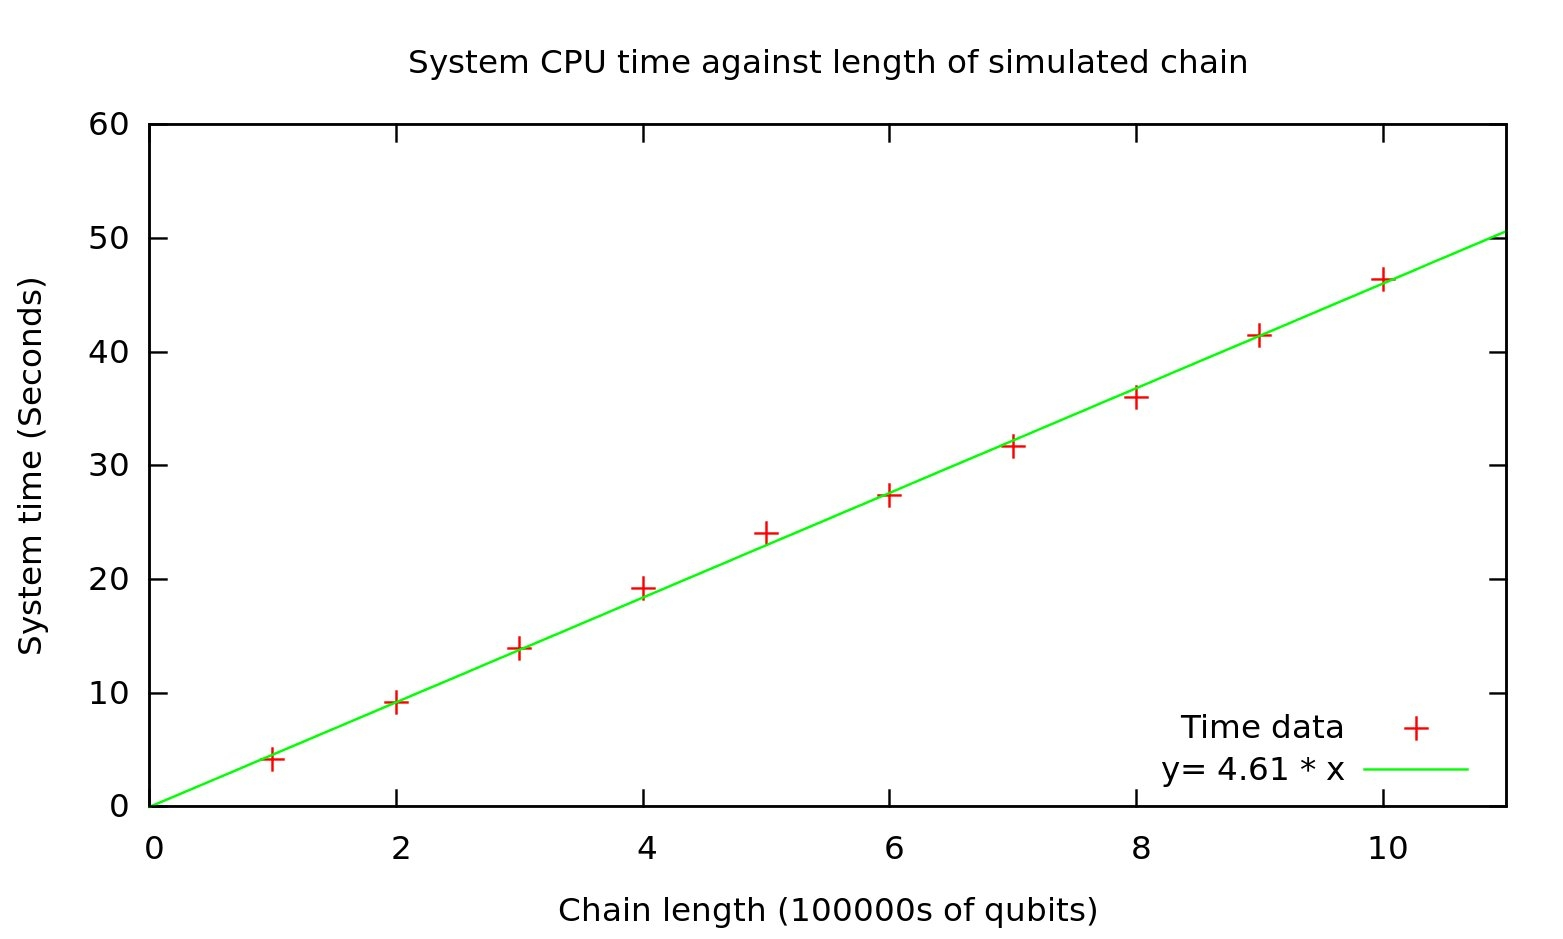
\includegraphics[scale=0.20]{gfx/singlechain_time_graph.jpg}
\caption{Graph of system CPU time against length of simulated chain for the SVD measurement method \label{fig:length_v_time_1}}
\end{figure}

In figure \ref{fig:length_v_time_1}, it can be seen that this relationship for the SVD method that removes qubits after each measurement has a linear relationship between time and chain length. This is as expected as the maximum matrix size is constantly low so the memory requirements for the program will be far lower than the projection operator method that require larger state vectors to be stored in memory. This result supports the claim made in \textit{"Cluster-state quantum computation"} \citep{nielsen_cluster-state_2006}, where it is shown that measurements on a quantum state can be efficiently simulated by a classical computer.


\begin{figure}
\centering
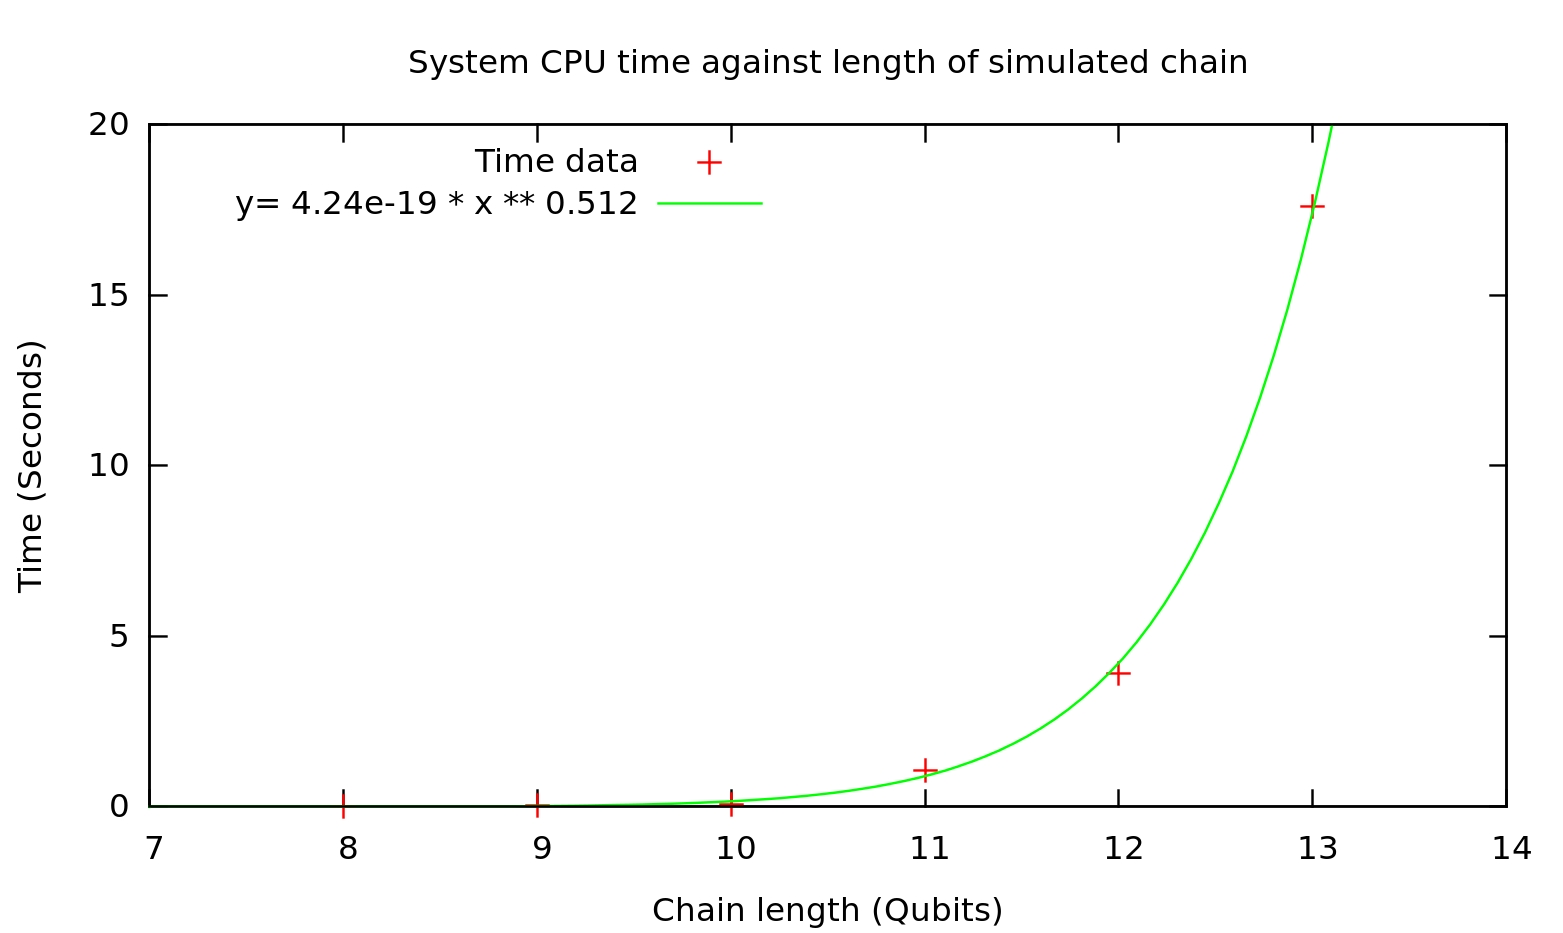
\includegraphics[scale=0.20]{gfx/timings2.jpg}
\caption{Graph of system CPU time against length of simulated chain for the projection operator measurement method \label{fig:length_v_time_2}}
\end{figure}

In figure \ref{fig:length_v_time_2} by contrast, it can be seen that the time scales approximately exponentially instead of the linear relationship from the previous figure. The parameters described in legend for the fitted curve are unlikely to be correct given the direction of the inflectional of the curve and are therefore best ignored. This implies a relationship of:

\begin{equation}
t \propto  \sim 2^{n}
\end{equation}


Which is as expected for the larger state vectors involved as the memory usage would need to scale in a similar manner which would explain the differences between the two simulations. This scaling is also indicative of the power of quantum computing because a real physical system would not have to scale in the same way allowing for efficient solutions to problems. When trying to simulate chains of larger than fourteen qubits in this manner the program seemed to time out before calculation, it is likely that this is because the program exceeded the memory limits of the machine so either more memory would be required to simulate larger systems or parts of the state vectors or operators would need to be stored on the hard disk, which would significantly bottleneck performance of the program.

The implications of this longer time extend onto future simulation of the error correction scheme which would require the same scaling factor when considering performance. Particularly as the simplest simulations of the error correction scheme would require at least six qubits to be simultaneously stored in memory along with their operators. However, as ten qubits can be fully simulated during the creation of cluster states and measurement in less than a second, simulations of the five qubit version of the error correction code would likely be able to be simulated easily for systems of two logical qubit. Unfortunately longer chains and multiple qubit gate operators would present a problem due to their significantly higher memory requirements given that they would likely require at least twenty five qubits which exceeds the current memory capacities of the machines used for simulation. In this case it would be necessary to use parallel processing to efficiently perform the simulation.


%----------------------------------------------------------------------------------------

\section{Conclusions}


While some progress was made in correcting problems with the program with measurements aside from the Pauli X measurement the goal of simulating the error correction scheme is still a long way from being achieved. The problem still seems to be present in the measurement itself given the in-correctness of the simulated Hadamard gate operation for all attempted methods of measurement simulation. It is therefore quite likely that there has been a fundamental misunderstanding of the theory behind the 'gate' operation itself which would need to be rectified for further progress to be made. Additionally there are clearly problems with the way by-product operators are calculated due to the mismatch between expected by-product and those used in the simulation and this will also have to be overcome or the operations required entered manually.

The investigations into the performance of the program did allow better insight into the kind of computational resources that would be required for simulation of the error correction scheme at least. It certainly seems that single logical qubit operations can be simulated with the same kind of hardware as used in this report while larger systems will require some orders of magnitude more. Hopefully this issue can be resolved for future versions of the program.
